 \subsection{Anticipated total duration of the project}

The anticipated duration of the project is three years (36 months).

\vspace{-1em}
\subsection{Objectives}
\label{sec:objectives}

The objective of this project is to develop approaches that address the six key challenges raised in \autoref{sec:startingpoint}. As shown in \autoref{fig:approach}, the first three approaches will 
focus on \emph{data transformation}, jointly allowing us to automatically turn a UI log into an event log, through event annotation, noise removal, and case identification. The latter three approaches will focus on process representation, turning an event log into an appropriate process model, through  abstraction, labeling, and visualization.

\begin{figure}[h!]
	\centering
	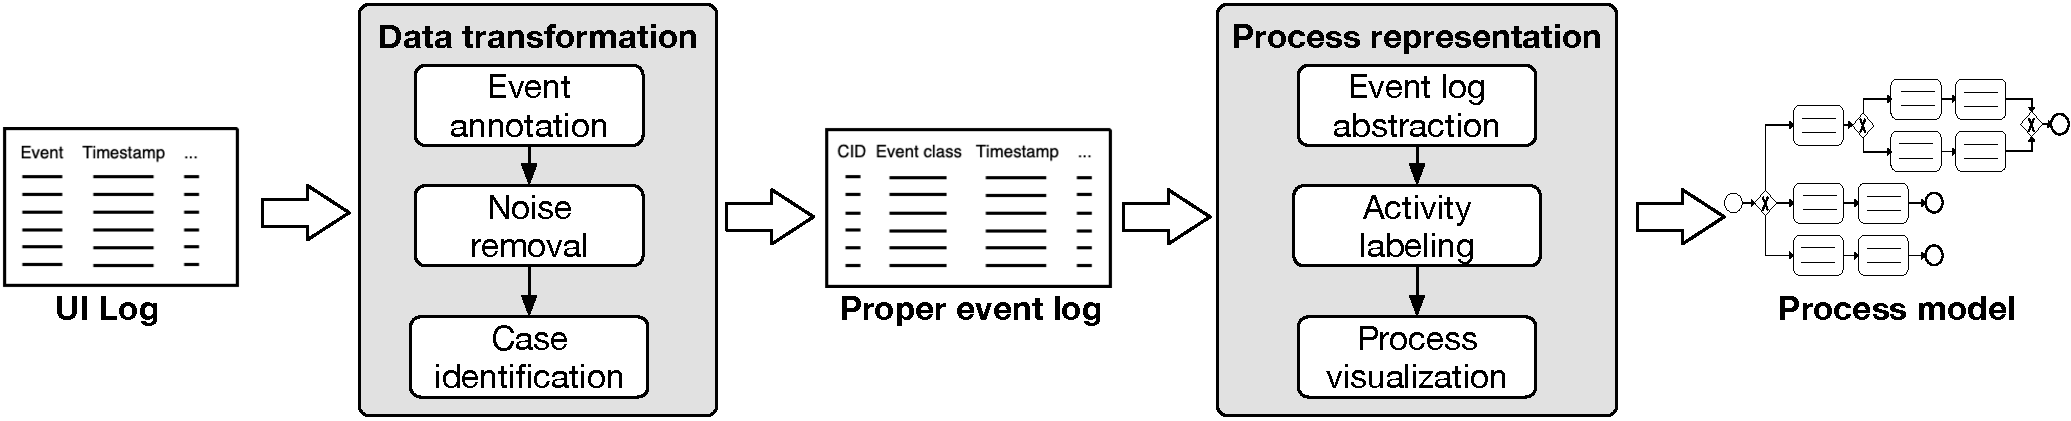
\includegraphics[width=\textwidth]{figures/overview.pdf}
	\caption{Overview of the proposed project}
	\label{fig:approach}
\end{figure}

\subsection{Work programme including proposed research methods}
\label{sec:workprogramme}

\mypar{Package structure} In accordance with the outlined objectives, we divided the work programme into two work streams (WS1 and WS2), encompassing a total of six work packages (WP1 to WP6). Stream WS1, focusing on data transformation, will be led by the University of Mannheim and consists of WP1 to WP3. Stream WS2, targeting process representation, will be led by the Kühne Logistics University and consists of WP4 to WP6. We have designed the two work streams in such a way that they can be executed independently from each other. We achieved this by ensuring that WS2 can build on publicly available,  event logs until the first results from WS1 are available. Therefore, both work streams can immediately start in parallel. 

\mypar{Research method} We will achieve our objectives through the design, implementation, and evaluation of novel process mining approaches. Their implementation will be conducted in Python, based on the \textit{PM4Py} process mining framework\footnote{\url{https://pm4py.fit.fraunhofer.de/}}. 
To evaluate the developed approaches, we will use publicly available data, such as the real-world UI logs  provided by the authors of \cite{leno2020identifying}\footnote{\url{https://figshare.com/articles/dataset/UI\_logs/12543587}} and widely-employed real-world event logs\footnote{\url{https://www.tf-pm.org/resources/logs}}.
Should we identify a need for evaluation data beyond publicly available logs, we will use the publicly available \textit{action logger}~\cite{leno2019action} tool to obtain additional UI logs. 
We will evaluate the approaches in WP1 to WP5 in terms of their \emph{accuracy} and \emph{efficiency}, e.g., with respect to manually established gold standards, whereas the \emph{usefulness} of the visualization approach developed in WP6 shall also be assessed through a user study. 

\vspace{-1em}
\subsubsection{WP1: UI log enrichment (6 PM)}
\label{sec:wp1}

While events in UI logs can be associated with a broad range of relevant attributes, they fundamentally lack the \emph{event labels} that are required in process mining to indicate the meaning of events or to recognize equivalent ones (by using labels to define \emph{event classes}).
To illustrate this, consider the shortened version of our UI log in \autoref{fig:example_short}. 
In an event log with proper labels, event 1 would carry a label such as ``\textit{Receive order}'', given that this is the event's main role in the process. Instead, the UI log only explicitly captures that the event was a ``\textit{click}'' on a ``\textit{list}'' in the application ``\textit{Outlook}''. That this click relates to receiving an order from a customer can only be inferred from the associated e-mail. 
Events 4 and 14 also highlight the importance of proper event labels for classifying events. Looking at the values of the key \textit{Event}, \textit{Application}, \textit{Element label}, and \textit{Element type} attributes, they appear to be identical. However, in fact, event 4 leads the user to a log-in screen (password entry succeeds the event), while event 14 completes the log-in process (password entry precedes the event). Proper labels could have clarified this difference, ensuring that these are considered as distinct steps in the process. 

The problem is that this labeling task is complex in reality. For example, only the \textit{URL} attribute helps to recognize that the specific application context differs between events 4 and 14.
In contrast, it may also be hard to recognize that certain events actually do relate to a similar context. For instance, events 4 and 7 both relate to activities in Salesforce, though their URLs differ considerably. At other times, as seen for event 1, labeling information needs to be derived from free-text attribute values, such as the contents of a message.

% For example, consider events 4, 7, and 13. According to the UI log, these events all occurred in the context of the application ``\textit{Chrome}'', i.e., an Internet browser. However, a brief analysis of the respective URL attributes reveals that event 4 relates to Salesforce and event 13 relates to Facebook. The fact that event 7 also relates to Salesforce is actually hard to identify since the URL structure of Salesforce changes once the user has logged into the application. 

\begin{figure}[h!]
	\centering
	\begin{adjustbox}{max width=\textwidth}
		\begin{tabular}{llllllll}
			\hline\noalign{\smallskip}\noalign{\smallskip}
			\textbf{ID} &\textbf{Timestamp}&\textbf{Event}&\textbf{Application}&\textbf{Element label}&\textbf{Element type}&\textbf{Element value}&\textbf{URL}\\
			\noalign{\smallskip}\hline\noalign{\smallskip}
			1&08:35.2&click&Outlook&Customer X - O123&list&Please initiate an order …&-\\\noalign{\smallskip}
			...&...&...&...&...&...&...&...\\
			4&08:39.7&click&Chrome&Log in&button&-&https://www.salesforce.com/\\\noalign{\smallskip}
			5&08:40.0&change&Chrome&Password&text field&-&https://login.salesforce.com/\\\noalign{\smallskip}
			6&08:40.5&click&Chrome&Submit&button&-&https://login.salesforce.com/\\\noalign{\smallskip}
			7&08:52.6&click&Chrome&New Account&button&-&https://com.lightning.force.com/home\\\noalign{\smallskip}
			...&...&...&...&...&...&...&...\\
			13&08:40.0&change&Chrome&Password&text field&-&https://www.facebook.com/\\\noalign{\smallskip}
			14&08:42.9&click&Chrome&Log in&button&-&https://www.facebook.com/\\\noalign{\smallskip}
			15&08:42.9&click&Chrome&Messenger&button&-&https://www.facebook.com/\\\noalign{\smallskip}
			...&...&...&...&...&...&...&...\\
			\hline\noalign{\smallskip}
		\end{tabular}
	\end{adjustbox}
	\caption{Shortened version of UI log from \autoref{fig:example}}
	\label{fig:example_short}
\end{figure}

To overcome this limitation in UI log data, this work package sets out to develop an approach for the semantic annotation of UI events. Specifically, we aim to enrich raw event data with additional labels, such that it is clear \textit{what} happened and \textit{where}. 
%Given that we intend to build on the semantics of the UI log events, we need to respectively enrich the raw event data from UI logs with additional labels such that it is clear \textit{what} happened and \textit{where}. 

\mypar{Semantic annotation - What} Available process analysis techniques leveraging semantics (e.g., \cite{leopold2012probabilistic,leopold2015_jss,van2021natural}) typically expect that each event can be associated with at least one \textit{action} and at least one \textit{business object}. Building on the example introduced above, the action for event 1 is ``\textit{receive}'' and the business object is ``\textit{order}''. While there are several techniques to derive actions and business objects from labels \cite{leopold2012refactoring,leopold2019using,rebmann2021extracting}, we need to infer these components from the available UI attributes. Therefore, we will develop a process-specific feature extraction technique, which identifies those textual attributes that have the specific roles of actions and business objects. To achieve this, we will combine and adapt existing techniques for the recognition of semantic process components in textual attributes~\cite{rebmann2021extracting} and the extraction of actions from free-text log attributes~\cite{gupta2020analyzing}. Specifically, we will first use graph-based topic discovery algorithms, such as CorePhrase \cite{hammouda2005corephrase}, to detect which attributes carry relevant information. Then, we will use a tagging mechanism based on BERT \cite{Devlin2019} to identify relevant actions and business objects. 

\mypar{Semantic annotation - Where} In traditional event logs, the application in which an event occurred is typically clear. That is, because the application itself records the occurrence of the event. In UI logs, the recording of the event is conducted independently of the used application(s). While the active application is captured in the \textit{application attribute} of the UI log, more and more business applications are browser-based (e.g. Salesforce, Office 365, Basecamp). Hence, the actual \textit{sub application} of many events must be inferred from the associated URL. To achieve this, we mainly build on string matching techniques. First, we check whether the application from the \textit{application attribute} is an Internet browser, which can be accomplished by consulting, e.g., the 
MediaWiki Action API\footnote{\url{https://www.mediawiki.org/wiki/API:Main_page}}. If this is the case, we resolve the URL via string matching. To illustrate this, consider event 4 from \autoref{fig:example}. After removing URL-specific prefixes and suffixes, we obtain ``\textit{salesforce}'', which can be easily verified as a business application using public resources. For events where this strategy does not deliver a conclusive result, we look at the event context. For example, for event 7, the string matching strategy is unlikely to deduce that this event occurred in Salesforce. However, when taking the log's context into account, we can clearly identify a number of sub applications, such as Salesforce (from event 4) and Facebook (from event 13). Although the URL of event 7 is rather cryptic, a string matching against these two available options, would clearly identify Salesforce as the most likely sub application. In this way, we resolve URLs and enrich the UI log with the specific application in which each event occurred, allowing downstream tasks to analyze events per context.

\mypar{Outcome} The outcome of this work package is an approach that enriches the UI logs with three new attributes, capturing \textit{actions}, \textit{business objects}, and \textit{sub application}. These additional attributes serve as an important basis for the application of existing process mining techniques and for the semantic analyses conducted in the subsequent work packages.  


\subsubsection{WP2:  Noise removal (13.5 PM)}
\label{sec:wp2}

UI logs often contain events that do not relate to the business process under investigation, such as events related to private activities (e.g., checking Facebook) or to non-related business activities (e.g., filing a reimbursement form of a business trip).
Given that process mining techniques assume that the events in a log relate to a single process, these irrelevant events, also referred to as \emph{noise}, need to be identified and removed from a UI log.

While various noise detection techniques already exist (cf., \autoref{sec:stateoftheart}), these  inherently approach noise detection from a different angle. Particularly, they aim to detect process behavior that stands out in terms of frequency (such as rare occurrence of an order being accepted before it is created), i.e., they try to \emph{detect events that are behavioral anomalies}, e.g., caused by recording errors.
Instead, when dealing with UI logs, we need to \emph{detect events that do not relate to the process at hand}. 

\mypar{Semantic noise detection}
To tackle this task, we propose to develop a semantic noise detection approach tailored to the specifics of UI logs, which aims to classify events as \emph{process relevant} or not. 
To achieve this, we transform the textual attribute values associated with each event  into a feature vector, after applying standard preprocessing steps such as lemmatization and stop-word removal. In this manner, we encode both general event information in features, as well as process-specific information extracted in the previous step, i.e., the event's action, business object, and application.

Once events are transformed into such feature vectors, noise identification can be approached as either a single-class or a two-class classification problem, using state-of-the-art text classifiers, such as a fine-tuned BERT~\cite{Devlin2019} model. The former involves training a classifier that recognizes which events are related to a specific process, e.g., by assuming that the majority of events in a UI log are related to that. While such an approach thus would not require any user input, the classification accuracy may be improved in a two-class setting, where users explicitly label some events as process relevant and irrelevant, so that few-shot learning techniques can be employed~\cite{yu2018diverse}.

Although such classifiers can be used with just a UI log as input, we will also incorporate mechanisms that allow user to provide additional domain-specific information about the process at hand, such as textual documentation or (high-level) process models, which can help the classifier to better distinguish process-relevant from irrelevant events.

\mypar{Outcome}
The outcome of this work package is a classification approach that identifies irrelevant events in a UI log. The approach will be applicable without requiring any additional user input, though users may improve the approach's accuracy by providing manually classified events or process-specific artifacts (e.g., a process model) as input.

\subsubsection{WP3: Case identification (16.5 PM)}
\label{sec:wp3}

Once irrelevant events have been filtered out from  a UI log, we next need to recognize which events belong to the same process instance, e.g., to the same customer order or service ticket, a task referred to as \emph{case identification}.

Existing techniques that address this task in general process mining settings primarily base the identification on co-occurrence statistics, which reveal behavioral regulations in an event log (cf., \autoref{sec:stateoftheart}). While such techniques work well for relatively structured settings, their performance deteriorates for event data stemming from more flexible environments, in which the execution of several cases overlap. This is, e.g., seen in the example of \autoref{fig:example}, where the first three events each start a new process instance, by initiating three different orders in a batch-like manner.

\mypar{Instance-based event matching}
Recognizing this challenge, this work package sets out to develop a new approach for case identification, tailored to the specifics of UI logs, by building on semantic matching technology.
Specifically, to determine the likelihood that events belong to the same case from a semantic viewpoint, e.g., because both refer to a same order ID or mention the same customer name, we frame the comparison of the events as an \emph{instance-based schema matching} task. For this, we recognize that events stemming from a particular application can be represented as instances in a particular schema (characterized by their payload attributes), enabling the application of existing matching techniques (cf., \cite{rinaldi2018matching,lehmberg2017stitching}).

\mypar{Optimization} Having obtained similarity scores between individual events, these scores can then be used together with behavioral regularities identified by existing techniques~\cite{diba2020extraction,ferreira2009discovering}, and cardinality constraints (e.g., each event belongs to exactly or at most one case), to establish an optimization problem, specifically using Markov logic formulation. By solving this problem, we will obtain an event grouping that maximizes the semantic similarity and respects the identified behavioral regularities for each of the identified cases.

\mypar{Outcome}
The outcome of this work package is a case identification approach that assign case identifiers to the events in a (filtered) UI log, such that the new log encompasses a number of cases, each corresponding to a sequence of events related to the same process instance. This, then, completes the transformation from a UI log into an event log suitable for process mining.


\subsubsection{WP4: Event abstraction (12 PM)}
\label{sec:wp4}

Even after transformation into a proper event log, the logs stemming from UI recordings comprise low-level event data, in which each event corresponds to a small action performed by a user. This fine-granular nature makes the data unsuitable for meaningful process analysis. This particularly holds for process discovery, since the application of discovery techniques on low-level event logs yields so-called \emph{spaghetti models}, as e.g., depicted in \autoref{fig:spaghetti}.

\begin{wrapfigure}{r}{0.5\textwidth} 
	\vspace{-15pt}
	\begin{center}
		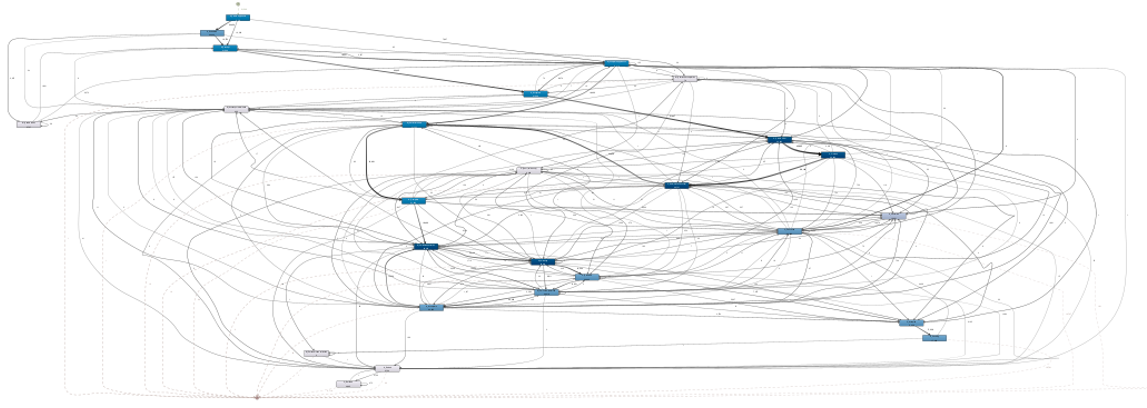
\includegraphics[width=\linewidth]{figures/spaghettiprocess.png}
		\caption{A so-called spaghetti process model}
		\label{fig:spaghetti}
	\end{center}
	\vspace{-15pt}
	\vspace{1pt}
\end{wrapfigure} 

To tackle this issue, event abstraction is a commonly used means to lift the event sequences of a log to a more abstract representation, by grouping low-level events into high-level activities. 
As discussed in \autoref{sec:stateoftheart}, various techniques for this purpose exist. Yet, their focus is on \emph{how} the abstraction is conducted, rather than \emph{what properties} the abstracted log shall satisfy. Without dedicated control on the result of event abstraction, however, it is hard to ensure that an abstraction is appropriate for a particular context or specific analysis goal.
This is particularly problematic in the context of UI logs, since these have clear characteristics that should or can be exploited to guide the abstraction task.

\mypar{Constraint-driven event abstraction}
To overcome this limitation, we propose to develop an approach for \emph{constraint-driven event abstraction}, which it supports a declarative characterization of the properties the abstracted log shall adhere to, in order to be meaningful for downstream analysis. While our approach shall support a broad range of constraint types, common ones to impose in the context of UI logs are for instance constraints that ensure that each high-level activity only comprises events that stem from the same application (to ensure semantic cohesion) or occurred within a certain timespan of each other (to ensure behavioral cohesion). 

Given such a set of user-defined constraints, our approach will aim to identify an optimal log abstraction, which groups together low-level event classes into high-level activities, such that a certain distance function, quantifying the behavioral and semantic similarity of events in an activity, is maximized, while still meeting the imposed constraints.

\mypar{Solution algorithms}
To guarantee an optimal solution, we will initially develop an approach for exhaustive log abstraction. Yet, striving for more efficient processing, we will also provide a heuristic version that is guided by behavioral dependencies found in the log, e.g., by recognizing certain event classes that shall never be grouped into a single activity, due to their relative positions in traces.
As such, this heuristic version shall aim to considerably improve the computation time, with limited impact on the quality of the obtained results.

\mypar{Constraint suggestion}
Although it is clear that guaranteeing user-defined constraints can lead to meaningful event abstraction, it may not always be obvious to users which constraints they shall request. Therefore, we will also develop an exploratory algorithm that strives to suggest \emph{interesting} constraints on the event data, such as particular attribute values that lead to a clear separation between different groups of events from a control-flow or temporal perspective, e.g., by considering aspects such as cohesion and coupling over the  abstracted log~\cite{vanderfeesten2007quality}. 
A prime challenge here would be to obtain suggestions in a computationally efficient manner, given the high dimensionality of the task. We aim to deal with this by reducing the problem size through decomposition of the event data, e.g., on the directly-follows graph, and by considering the characteristics of data attributes in the log, e.g., through data profiling~\cite{papenbrock2015data}, allowing us to discard unpromising attributes in advance.


\mypar{Outcome} The outcome of this work package is an approach that allows users to abstract a low-level event log into high-level activities based on user-defined or suggested abstraction requirements, providing clear insights into the high-level process behavior contained in the UI log.


\subsubsection{WP5: Activity labeling (12 PM)}
\label{sec:wp5}

The value of a discovered process model highly depends on the quality of its activity labels, since these labels form the basis of what a human can understand about the process~\cite{mendling2010activity,Leopold2013Book}. Recognizing this,  the importance of clear and informative labels in process models has led to a large body of literature concerned with labeling guidelines~\cite{mendling2010seven,leopold2015learning} and their automatic enforcement~\cite{leopold2013detection,becker2009towards}. 
These best practices indicate that process model activity labels should contain an action provided as an imperative verb (e.g. ``\textit{create}" or ``\textit{send}'') and at least one business object provided as a noun (e.g. ``\textit{order}'' or ``\textit{e-mail}''). Additional information can be provided at the end of the label if required. Following these rules results in labels such as ``\textit{Create order}'' or ``\textit{Send e-mail to customer}''. 

The challenge in the context of this work package is to automatically generate meaningful labels for each group of UI events that has been identified in the event-abstraction step (WP4). To illustrate this, consider the events 4, 5, and 6 from the UI log in \autoref{fig:example}, which, respectively, refer to the pressing of a log-in button, entering a password, and pressing the submit button.
Recognizing the joint role of these events in the process, a proper label for the group could be ``\textit{Log into Salesforce}", which summarizes both the outcome (logging in) and the context (SalesForce) of the event group. 
However, automatically generating such \textit{higher-level labels} is complex, since it requires to infer an overarching activity from the actions, business objects, and application contexts of multiple low-level events. Furthermore, how to derive such an overarching label depends on the nature of the events and, thus, differs per situation. Therefore, we propose different strategies:

%the action, business object, and (sub) application attributes.

\mypar{Labeling strategies} To generate higher-level labels, we jointly analyze the behavioral and semantic perspectives of grouped events, resulting in three different strategies. Building on the observations from early work on process model name generation~\cite{leopold2014simplifying}, we distinguish three specific strategies: 1) outcome-oriented labeling, 2) decision-based labeling, and 3) holonym-based labeling. 

The \textit{outcome-oriented labeling} strategy can be applied if the considered group of UI events has a clear result that can be used to described the previous steps. An example of this is the aforementioned ``\textit{Log into Salesforce}" label for events 4, 5, and 6.
%
The \textit{decision-based labeling} strategy builds on the fact that many processes are driven by key decisions being made, such as deciding to reject or accept an offer from a customer. If a considered group of events encompasses such a decision point, this can be used as the main information captured in a label, such as ``\textit{Decide about customer offer}''. 
%
Finally, the \textit{holonym-based labeling} strategy is applied to situations where low-level events jointly contribute to a higher-level activity. In linguistics, a \textit{holonym} is a term that has a part-of relation with a number of \textit{meronyms}, e.g., a ``\textit{finger}'' is a meronym of the holonym ``\textit{hand}''.
By applying the notion of holonymy to events, we aim to recognize action or business objects that are considered to be meronyms, allowing us to detect the holonym describing the higher-level activity. As an example, consider events 11, 12, and 13 from \autoref{fig:example}. While these events are essentially copy and paste operations, they all contribute to a higher-level event that could be described as ``\textit{Create customer account in Salesforce}''. 

We shall turn each of these strategies into an automated label-generation technique. This involves dealing with specific challenges caused by the process-specific nature of data our project deals with. For example, with respect to the latter strategy, existing work has tried to address the problem of holonymy detection on process model activities by building on WordNet~\cite{leopold2014simplifying}. Yet, while WordNet is useful to detect general-purpose holonymy relations (such as between ``\textit{finger}'' and ``\textit{hand}''), it fails to detect more complex and domain-specific relations commonly found in process-mining contexts. Therefore, we will leverage techniques from ontology learning~\cite{al2020automatic,wong2012ontology} to automatically derive holonymy relations from general and domain-specific text corpora.    

\mypar{Strategy selection} The three strategies can result in different labels for the same group of events. Therefore, aside from developing the labeling strategies themselves, we will also develop a decision mechanism that will select the most appropriate strategy for a specific group, building on both behavioral and semantic analysis of the low-level events. For example, the decision-based strategy shall be employed when the behavioral relations indicate a choice in the process, e.g., signaled by mutually exclusive events, or when low-level actions have clearly opposite meanings, e.g., \emph{reject} versus \emph{accept}. Similarly, the outcome-oriented strategy shall be employed if the group of events represents a synchronization point in a process, such as a \emph{log-in step}, which is succeeded by various other paths. Finally, the holonym-based strategy shall be reserved for situations where such holonym relations can actually be identified for the low-level events. 

\mypar{Outcome} The outcome of this work package is an approach that, given a group of UI events, automatically selects the appropriate labeling strategy for this group and applies it to obtain a higher-level activity label. These labels are then used as additional annotations for the log stemming from WP4, resulting in an abstracted and meaningful event log. 

% technique that creates an event log with properly labeled higher-level events, i.e., labels consisting at least of an action and a business object. This event log serves as input for the technique from work package 6. 

\subsubsection{WP6: Visualization (12 PM)}
\label{sec:wp6}

The final step is concerned with the visualization of the process captured in the UI log. In traditional process discovery, this is achieved by generating respective process models. Depending on the employed discovery algorithm, the resulting process model is a simple directly-follows graph \cite{van2019practitioner}, a Petri net \cite{van2004workflow}, a BPMN model \cite{conforti2016bpmn}, or a process tree \cite{leemans2013discovering}. While each algorithm and output representation come with advantages and disadvantages, there is no specific discovery technique available for the UI log generated in WP1 to WP5. The specific challenge is that the original level of granularity of the UI log is not appropriate for visualization since the number of events is too high. Yet, the user might be interested in getting insights into this level to fully understand how the process is executed. What is required is a discovery algorithm that allows the user to adapt the process visualization in a flexible manner with respect to 1) the abstraction level and 2) the general scope. In the context of data warehousing and OLAP \cite{chaudhuri1997overview}, the former corresponds to \textit{drilling down} and \textit{rolling up}, while the latter corresponds to \textit{slicing}. 

\mypar{Slider-based abstraction} The general idea of adapting the level of abstraction using a slider approach is present in several commercial process mining tools, such as Celonis\footnote{\url{www.celonis.com}} and Disco\footnote{\url{https://fluxicon.com/disco/}}. However, they implement abstraction by removing arcs or nodes based on their frequency. Our idea is to merge events based on the abstraction mechanism introduced in WP4 and use the approach from WP5 to present meaningful labels to the user. In case the user is interested in more details, the user can drill down on individual events or groups thereof and explore the process on several levels at the same time. To this end, we will build on the ideas on multi-level discovery from \cite{leemans2020using} and adapt them to the specific scenario of slider-based abstraction. 

\mypar{Semantic scoping} Besides adapting the level of abstraction, the user might also want to modify the general scope of the discovered model. It is well imaginable that, for instance, there are specific applications or business objects in the process the user wishes to investigate further or, in the opposite case, remove them from the visualization. We, therefore, introduce a scoping  mechanism that allows the user to select applications and business objects that should be included or removed. We then leverage semantic technology to determine which events should be included or removed from the presented model. Note that this is not trivial since the links between applications and business objects are complex and simply removing all events that do not mention the selected term ``\textit{invoice}'' is certainly too simplistic. Hence, we determine which other events are semantically related to selected business object(s) and respectively include them, while simultaneously ensuring the correctness of the scoped process from a behavioral perspective.    

\mypar{User evaluation} The two mechanisms introduced above are novel and require interaction with users. Therefore, we plan to complement the technical evaluation of our approach with a user study. Specifically, we aim to investigate the effectiveness (in terms of the ability of obtaining insights) and efficiency (in terms of how fast user can obtain insights).  For this, we will build on our experience with user studies in the context of process understandability~\cite{pittke2015automatic} and process modeling support~\cite{van2020say}.

\mypar{Outcome} The outcome of this work package is a novel discovery and representation approach that can visualize UI logs in a flexible fashion. As such, it completes our overall pipeline for semantic process elicitation and discovery from UI logs.  



\subsubsection{Overview on the work plan}

\begin{figure}[bt]
	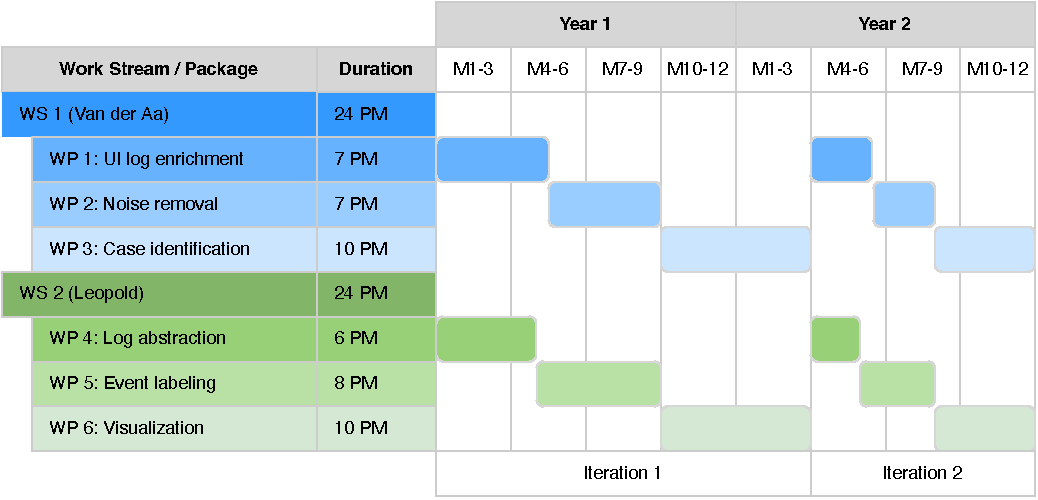
\includegraphics[width=\textwidth]{Figures/Gantt.pdf}
	\caption{Work plan}
	\label{fig:workplan}
\end{figure}

As explained above, the project consists of two work streams and six work packages. Naturally, there are interdependencies among these work packages. Figure \ref{fig:workplan} shows a simplified work plan that mostly abstracts from parallel and overlapping work within each work stream. It is important to highlight that the transitions between two packages will not be as strict as depicted. We are aware of the various interdependencies and will take them into account appropriately.  
There are, for instance, interdependencies between WP1 and WP1. Without an enriched UI log, the noise removal technique cannot build on the newly introduce attributes. This, however, can be addressed by taking the manually created gold standard for the evaluation of WP1 as input for WP2. In this way, the noise removal technique cannot already be developed without needing a ``perfect'' solution for WP1. The rather abstract view on the work plan shown in Figure \ref{fig:workplan} highlights our general idea of having two main iterations:
\begin{itemize}
	\item The first iteration ends after 21 months. At the end of this iteration, there will be a first implemented prototype available. The individual techniques have been evaluated both independently and as a whole. The main outcome from this iteration, therefore, are insights into the strengths and weaknesses of our techniques, which allows us to determine the required improvements and adaptations for the second iteration. 
	\item The second iteration is slightly shorter and will be mainly used to address identified weaknesses and improve the performance of the technique.
\end{itemize} 

Note that these two iterations also help us to account for the interdependencies between the two work streams (as discussed earlier). In the first iteration, WS 2 will build on traditional, freely available event logs, while in the second iteration WS 2 can build on a UI log that has been processed with the techniques from WS1. 



%Note that the work plan shown above allocates a total of 42 project months to 3 years. As explained in Section \ref{sec:staff}, we intend to hire a PhD student for 3 years, which means that remaining 6 project months will be covered by the respective principal investigator of this project. 